
\section{Descripción}

\paragraph{}
El proyecto consiste en un juego de carreras en dos dimensiones con vista cenital, en el que se podrá competirá contra la 
inteligencia artificial. 
La idea es realizar un juego entretenido y dinámico, que estará compuesto por varios modos de juego.

\begin{figure}[H]
  \label{logo_zycars}
  \begin{center}
    
\includegraphics[scale=0.5]{imagenes/logo_zycars.png}
  \end{center}
  \caption{Descripción: Logo de Zycars}
\end{figure}

\section{Características del videojuego}

\paragraph{}
El videojuego ofrece una alternativa libre, gratuita y original para jugar a un juego de conducción en dos dimensiones. 
Las posibilidades que ofrece son las siguientes:

\subsection{Modos de juego}

\paragraph{}
En \emph{Zycars} tendremos distintos modos de juegos, en cada uno de ellos el
objetivo que habrá que llevar a cabo será distinto.
A continuación se describirán los distintos modos de juegos que tendrá el videjuego:

\subsubsection{Carrera rápida} 

\paragraph{}
El juego en el modo de carrera rápida ofrece la posibilidad de enfrentarnos a 3 personajes 
controlados por la inteligencia artificial, a lo largo de un circuito que
hayamos seleccionado previamente. El número de vueltas
que se realicen durante la carrera estarán a elección del jugador y se podrá elegir el número de las mismas a la hora de seleccionar
el circuito.

\subsubsection{Campeonato} 

\paragraph{}
En este modo de juego podremos competir contra 3 personaje controlados por la inteligencia artificial 
a lo largo de un campeonato completo, el cual habremos elegido previamente. 

\paragraph{}
El campeonato estará compuesto por cuatro circuitos y el número de vueltas a estos, también estarán a elección del jugador 
al igual que en el modo de juego explicado anteriormente.

\paragraph{}
Tras la conclusión de cada una de las carreras, los jugadores obtendrán una puntuación en función de la posición que haya 
obtenido. El jugador que mayor puntuación haya conseguido tras acabar los cuatro circuitos, se proclamará ganador del 
campeonato.

\subsubsection{Contrarreloj} 

\paragraph{}
En este último modo de juego y a diferencia de los dos anteriores, el jugador competirá solo sin la ningún oponente.

\paragraph{}
El objetivo en este modo de juego será la realización de los circuitos ofrecidos y mejorar los tiempos de estos, ya sean la 
vuelta más rápida del circuito o el tiempo general. El número de vueltas que deberemos dar al circuito será un total de tres, a
diferencia de los modos anteriores, no tendremos la posibilidad de modificar el valor.

\subsection{Elementos de juego}

\paragraph{}
En esta sección se hará una pequeña descripción de los distintos elementos que encontraremos a lo largo del juego, ya sean 
manipulados por los jugadores, o encontrados a lo largo de los circuitos.

\subsubsection{Personajes}
	
\paragraph{}
Los elementos básico del juego, habrá disponibles distintos personajes que tendrán asociado un 
vehículo característico a su personalidad y apariencia. Cada uno de ellos
tendrán distintas características, 
cosa a tener en cuenta a la hora de hacer nuestra elección por uno de ellos, como la velocidad, la aceleración y el giro.
	
\begin{figure}[H]
	\label{ejemplo_personaje2}
	\begin{center}
		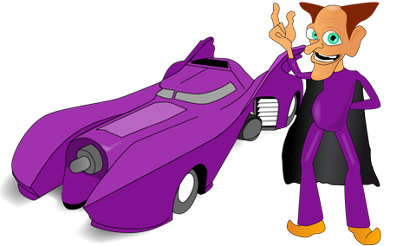
\includegraphics[scale=0.7]{imagenes/ejemplo_personaje2.png}
	\end{center}
	\caption{Descripción: Personaje de Zycars.}
\end{figure}

\subsubsection{Cajas de ítems} 

\paragraph{}
A lo largo de los circuitos en los que estemos compitiendo contra la inteligencia artificial, 
podremos encontrar distintas cajas que al colisionar con ellas nos proporcionen
aleatoriamente una habilidad o ítem que nos
ayuden en la competición contra nuestros rivales.

\begin{figure}[H]
	\label{item_box}
	\begin{center}
		
\includegraphics[scale=1]{imagenes/items/item_box.png}
	\end{center}
	\caption{Descripción: Caja de ítem.}
\end{figure}

\subsubsection{Tipos de ítems}

Los ítems que podremos obtener a partir de la caja de ítems, los podremos diferenciar principalmente en tres tipos:

\begin{description}
	\item \textbf{Ataques a distancia} Estos nos permitirán lanzar ataques
        de forma que podamos interceptar a los competidores que 
	se encuentres lejos de nosotros.
	
	\item \textbf{Obstáculos} Estos nos permitan dejar obstáculos en el
        recorrido, que reduzcan nuestra velocidad considerablemente
	o aquellos que al pasar por encima perdamos completamente el control de nuestro vehículo por unos instantes de tiempo.
	
	\item \textbf{Velocidad} Esto nos darán la opción de aumentar nuestra velocidad durante un pequeño intervalo de tiempo.
\end{description}
